% Created 2021-01-02 sam. 19:03
% Intended LaTeX compiler: pdflatex
\documentclass[twocolumn]{scrartcl}

% \KOMAoptions{
%   numbers=noenddot,
%   DIV=12}
\usepackage{scrhack}
\setlength\footskip{3em}
%\usepackage[bottom=30mm,top=30mm,inner=35mm,outer=30mm]{geometry}
%%%%%%%%%%%%
% Language %
%%%%%%%%%%%%

\usepackage{subfiles}
\usepackage[german,french,english]{babel}
\usepackage[utf8]{inputenc} % encodage
\usepackage[T1]{fontenc}

\usepackage[abbreviations,british]{foreign}
\usepackage{setspace}
\usepackage[babel=true,activate={true,nocompatibility},final,tracking=true,kerning=true,factor=1100,stretch=10,shrink=10]{microtype}


%%%%%%%%%%%%%%%
% References  %
%%%%%%%%%%%%%%%
\usepackage[dvipsnames,x11names]{xcolor} % Un peu de couleur !
\usepackage{float}
\usepackage{subcaption}
\usepackage{hyperref}
\hypersetup{
    unicode=true,            % non-Latin characters in Acrobat’s bookmarks
    pdftoolbar=true,         % show Acrobat’s toolbar?
    pdfmenubar=true,         % show Acrobat’s menu?
    pdffitwindow=false,      % window fit to page when opened
   % pdfstartview={FitH},     % fits the width of the page to the window
   % pdftitle=\@title,      % title
  %  pdfauthor=\@author,    % author
    colorlinks=true,         % false: boxed links; true: colored links
    linkcolor=black,      % color of internal links
    citecolor=OliveGreen,    % color of links to bibliography
    filecolor=magenta,       % color of file links
    urlcolor=BlueViolet      % color of external links
}
\usepackage[backend=biber,
sorting=none]{biblatex}

\addbibresource{articles/audioDeclipping.bib}

\usepackage{mathtools}
\usepackage{bbold}
\usepackage{mathrsfs}
\usepackage{amssymb}
\usepackage{amsbsy}
\renewcommand{\vec}[1]{\boldsymbol{#1}}

\author{Pierre-Antoine Comby}
\date{2020-12-07}
\title{A Review of audio declipping through a sparse prior}
\begin{document}

\maketitle
\begin{abstract}
  The inverse problem of audio declipping is ill posed and a regularization prior is thus needed, in particular a sparse synthesis (or in dual space a analysis) are presented and tested. In the following, we implement and extends the methods presented in \cite{kitic_sparsity_2015-1}
\end{abstract}

\section{The declipping problem}

The saturation of an audio signal occurs often in signal processing and communication, when the original or signal are not available, one requires to reconstruct the parts of the signal which have been lost.
We  consider an original signal \(\vec{x} \in \mathbb{R}^{N}\) which have been clipped to produced \(\vec{y}\).

\[y =
  \begin{cases}
    x_{i} & \text{ if }  \tau^{-} \le x_{i} \le \tau^{+} \\
    \tau^{+} & \text{ if }  \tau^{+} \le x_{i} \\
    \tau^{+} & \text{ if }  x_{i} \le \tau^{-}
  \end{cases}\]

Our goal is to retrieve \(\hat{\vec{x}}\), which is as close as possible from the original signal  \(\vec{x}\). An extensive review of the solution developed for this problem is done in \cite{noauthor_survey_nodate}, and references herein.

\subsection{Constrained Optimisation}
The indexes of \(\vec{y}\) can be separated into three sets:
\begin{itemize}
  \item \(\Omega_r = \{i \in 1,...,N | y_i = x_i \}\)
  \item \(\Omega_c^+ = \{i \in  1,...,N | y_i =  \tau^{+} \}\)
  \item \(\Omega_c^- = \{i \in 1, ..., N| y_i = \tau^{-} \}\)
\end{itemize}

A correct estimation of \(\vec{x}\)  should thus verify:

\begin{itemize}
  \item \(\hat{\vec{x}}(\Omega_r) = \vec{y}(\Omega_r)\)
  \item \(\hat{\vec{x}}(\Omega_c^+) \ge \tau\)
  \item \(\hat{\vec{x}}(\Omega_c^-) \le -\tau\)
\end{itemize}
These constraints are denoted as \(\hat{\vec{x}} \in \Gamma(y)\). \(\Gamma(\vec{y})\) is a convex set, and enforcing the previous constraint will be assured by projecting the candidates estimation on \(\Gamma\). Such projection can be implemented as follows:
\[ P_{\Gamma(\vec{y})}(\vec{x}) = \max(\min(\vec{x},\vec{\gamma}_{-}),\vec{\gamma}_{+})\]

With:
\[\begin{cases}
    \vec{\gamma}_{-}(\Omega_{r}) &= y(\Omega_{r}) \\
    \vec{\gamma}_{-}(\Omega_{c}^{-}) &= \tau^{-} \\
    \vec{\gamma}_{-}(\Omega_{c}^{+}) &= +\infty \\
  \end{cases} \quad
  \begin{cases}
    \vec{\gamma}_{+}(\Omega_{r}) &= y(\Omega_{r}) \\
    \vec{\gamma}_{+}(\Omega_{c}^{-}) &= -\infty \\
    \vec{\gamma}_{+}(\Omega_{c}^{+}) &= \tau^{+} \\
  \end{cases}\]

\subsection{Regularization through Sparsity}

The state of the art for the regularization is to use a sparsity (or in dual space, co-sparsity) prior to solve the inverse problem of declipping. Other approach that are also worth mentioning are: linear prediction, minimization of th energy of high order derivative and psycoacoustic.

The sparsity prior rely on a time-frequency analysis, (or synthesis in a dual framework). We consider the Analysis operator \(\vec{A}\), such that \(\vec{z} =\vec{Ax}\), with \(\vec{z}\) the sparse representation of \(x\) in a dictionnary space (e.g. a Gabor frame).
The \emph{Analysis Sparse Audio Declipper} (A-SPADE) Problem is  therefore:

\begin{equation}
  \label{eq:ASPADE}
  \arg\min_{x\in \mathbb{R}^{N}} \|z\|_{0} \text{ s.t. } \|\vec{Ax-z}\|_{2} \le \epsilon \text{ and } x\in \Gamma(\vec{y})
\end{equation}
Or on  the dual side, the Synthesis Sparse Audio Declipper (S-SPADE):
\begin{equation}
  \label{eq:SSPADE}
  \arg\min_{x\in \mathbb{R}^{N}} \|z\|_{0} \text{ s.t. } \|\vec{x-Dz}\|_{2} \le \epsilon \text{ and } x\in \Gamma(\vec{y})
\end{equation}

\section{Algorithms}
\subsection{ADMM}
Both  \eqref{eq:ASPADE} and  \eqref{eq:SSPADE} are solvable via the Alternating Direction Method of Multipliers (ADMM). ADMM can solve problem of the form
\begin{equation}
  \label{eq:ADMM}
  \begin{aligned}
    &\min_{\vec{x}} f(\vec{x}) + g(\vec{Ax}) \\
    &\iff \min_{\vec{x,z}} f(\vec{x})+g(\vec{z}) \text{ s.t } \vec{Ax}-z = 0
  \end{aligned}
\end{equation}
With \(f,g\)  two convex function and \(\vec{A}\) A linear operator. In our case we can write the A-SPADE and S-SPADE problem as:
\begin{equation}
  \label{eq:2}
  \arg\min_{x,z,k} \underbrace{\mathbb{1}_{l_{0}\le k}(z)}_{g(\vec{z})} + \underbrace{\mathbb{1}_{\Gamma(y)}(\vec{x})}_{f(\vec{x})}  \text{ s.t. } \vec{Ax}=\vec{z}
\end{equation}
\begin{equation}
  \label{eq:2}
  \arg\min_{x,z,k} \underbrace{\mathbb{1}_{l_{0}\le k}(z)}_{g(\vec{z})} + \underbrace{\mathbb{1}_{\Gamma(y)}(\vec{x})}_{f(\vec{x})}  \text{ s.t. } \vec{Dz}=\vec{x}
\end{equation}
With a fixed \(k\)  we identify an ADMM solvable problem, (but only locally, as the \(l_{0}\) norm is not a smooth convex function).

Consequently, we have the following iterative scheme for A-SPADE, derived from the solution for ADMM \cite{zaviska_s-spade_2020}

\begin{subequations}
  \label{eq:ASPADE-step}
  \begin{align}
    \vec{x}^{(i+1)}&=\underset{\vec{x}\in \Gamma(\vec{y})}{\operatorname{argmin}}\left\|A \vec{x}-\vec{z}^{(i)}+\vec{u}^{(i)}\right\|_{2}^{2} \\
    \vec{z}^{(i+1)}&=\underset{\vec{z}\in l_{0}\le k}{\operatorname{argmin}}\left\|A \vec{x}^{(i+1)}-\vec{z}+\vec{u}^{(i)}\right\|_{2}^{2}\\
    \vec{u}^{(i+1)}&=\vec{u}^{(i)}+A \vec{x}^{(i+1)}-\vec{z}^{(i+1)}
  \end{align}
\end{subequations}
and an analoguous one for S-SPADE \textbf{cite}:
\begin{subequations}
  \label{eq:SSPADE-step}
  \begin{align}
    \vec{z}^{(i+1)}&=\underset{\vec{z}\in l_{0}\le k}{\operatorname{argmin}}\left\|D \vec{z}-\vec{x}^{(i)}+\vec{u}^{(i)}\right\|_{2}^{2}\\
    \vec{x}^{(i+1)}&=\underset{\vec{x}\in \Gamma(\vec{y})}{\operatorname{argmin}}\left\|D \vec{z}^{(i+1)}-\vec{x}+\vec{u}^{(i)}\right\|_{2}^{2}\\
    \vec{u}^{(i+1)}&=\vec{u}^{(i)}+D \vec{z}^{(i+1)}-\vec{x}^{(i+1)}
  \end{align}
\end{subequations}
The hypothesis of a \(k\)-sparse vector is incrementally relaxed (e.g., $k \leftarrow k+1$ at each step). In the case \(\vec{D}^{\star} = \vec{A}\)  the two algorithm are completely equivalent, and S-SPADE is entirely the dual representation of A-SPADE: \(\vec{z}\) become the primal variable, and \(\vec{x}\) the dual one.


\subsection{Implementation}

Both minimization steps provide projection on a convex set. With the hypothesis of  a Parseveal frame  (\(\vec{A^{*}A}= \vec{I}\) or \(\vec{D^{*}D} = \vec{I}\)) we have
\begin{subequations}
  \label{eq:ASPADE-step2}
  \begin{align}
    \vec{x}^{(i+1)}&= P_{\Gamma(\vec{y})}(\vec{A}^{*}(z^{(i)}-u^{(i)}))\\
    \vec{z}^{(i+1)}&=\mathcal{H}_{k}(\vec{A}\vec{x}^{(i+1)}+\vec{u}^{(i)})\\
    \vec{u}^{(i+1)}&=\vec{u}^{(i)}+A \vec{x}^{(i+1)}-\vec{z}^{(i+1)}
  \end{align}
\end{subequations}
and S-SPADE:
\begin{subequations}
  \label{eq:SSPADE-step2}
  \begin{align}
    \vec{z}^{(i+1)}&=\mathcal{H}_{k}(\vec{D}^{*}(\vec{x}^{(i)}-\vec{u}^{(i)}))\\
    \vec{x}^{(i+1)}&=P_{\Gamma(\vec{y})}(\vec{D}^{*}(\vec{x}-\vec{u}^{(i)}))\\
    \vec{u}^{(i+1)}&=\vec{u}^{(i)}+D \vec{z}^{(i+1)}-\vec{x}^{(i+1)}
  \end{align}
\end{subequations}

The presented algorithm have been implemented using Python, and its modules Numpy and Scipy.
All the sources of this project are available at \url{https://gitlab.crans.org/comby/audioDeclipping}, bug report and improvements are welcome. A similar project using MATLAB, presented in \cite{zaviska_revisiting_2018} is also available at \url{http://www.utko.feec.vutbr.cz/~rajmic/software/aspade_vs_sspade.zip}. One should note, that at the time of writing this report, the MATLAB implementation performs better and faster. I prefer however to present hereafter my personal work. The use of python has been motivated by its ease of extensibility using Object Oriented Programming and encapsulation, its free and opensource licensing and its more and more frequent use in the signal processing community, it lacks however a module comparable to the LTFAT toolbox (a partial port of the toolbox exists)


\section{Results}
Unfortunately, the python implementation does not yields exactly the same results as the one presented in , and I assume that the computational time could be significantly reduced by using a more efficient STFT implementation (for example using the well known FFTW).

The quality measurement is done with the Signal-to-Distortion-Ratio \cite{kitic_sparsity_2015-1}
\begin{equation}
  \mathrm{SDR}_{\boldsymbol{y}}=20 \log _{10} \frac{\left\|\left[
        \begin{array}{c}
          \Omega_{\mathrm{c}}^{+} \\
          \Omega_{\mathrm{c}}^{-}
        \end{array}\right]
      \boldsymbol{x}\right\|_{2}}{\left\|\left[
        \begin{array}{c}
          \Omega_{\mathrm{c}}^{+} \\
          \Omega_{\mathrm{c}}^{-}
        \end{array}\right]
      \boldsymbol{x}-
      \left[\begin{array}{c}
              \Omega_{\mathrm{c}}^{+} \\
              \Omega_{\mathrm{c}}^{-}
            \end{array}\right] \boldsymbol{y}\right\|_{2}},
    \end{equation}

    \begin{equation}
      \mathrm{SDR}_{\hat{\boldsymbol{x}}}=20 \log _{10} \frac{\left\|\left[
            \begin{array}{c}
              \Omega_{\mathrm{c}}^{+} \\
              \Omega_{\mathrm{c}}^{-}
            \end{array}\right]
          \boldsymbol{x}\right\|_{2}}{\left\|\left[
            \begin{array}{c}
              \Omega_{\mathrm{c}}^{+} \\
              \Omega_{\mathrm{c}}^{-}
            \end{array}\right]
          \boldsymbol{x}-\left[
            \begin{array}{c}
              \Omega_{\mathrm{c}}^{+} \\
              \Omega_{\mathrm{c}}^{-}
            \end{array}\right]
          \hat{\boldsymbol{x}}\right\|_{2}}
    \end{equation}

\begin{figure*}
  \centering
 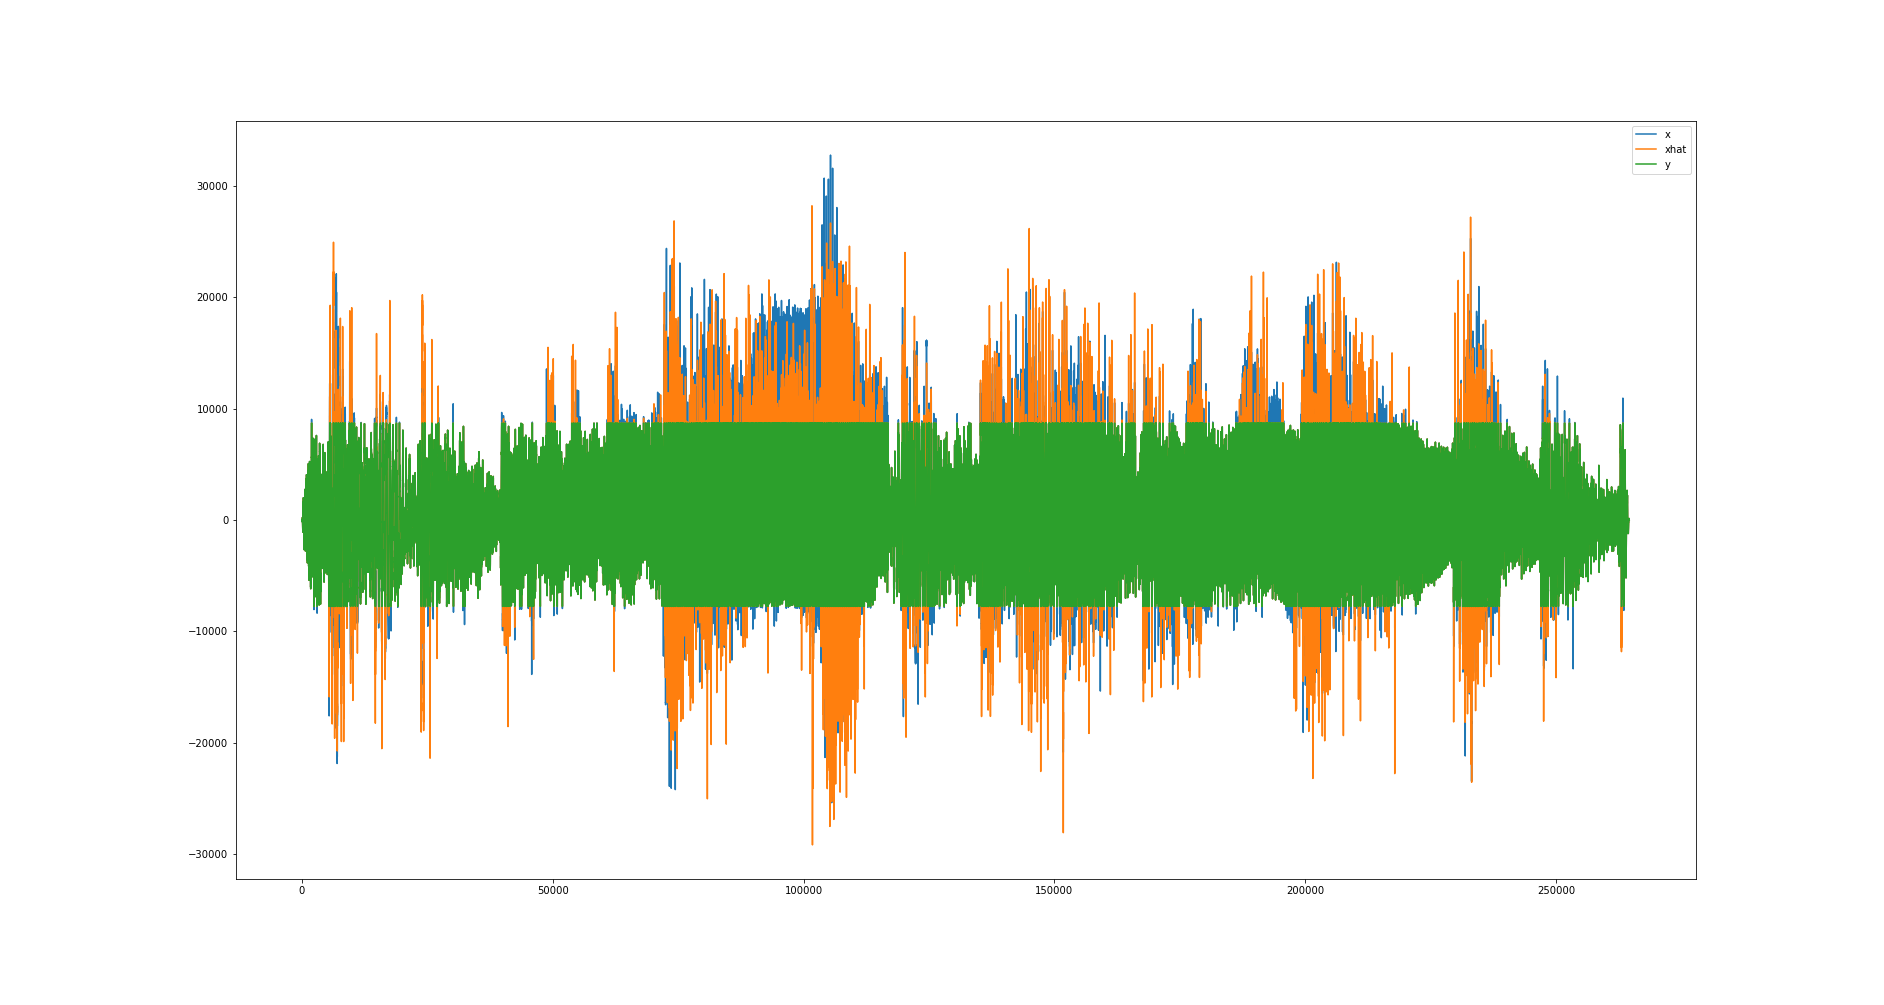
\includegraphics[width=\textwidth]{fig/Figure_2.png}
 \caption{Exemple of reconstruction using A-SPADE.}
 \label{fig:plot}
\end{figure*}
\begin{figure*}
  \centering
  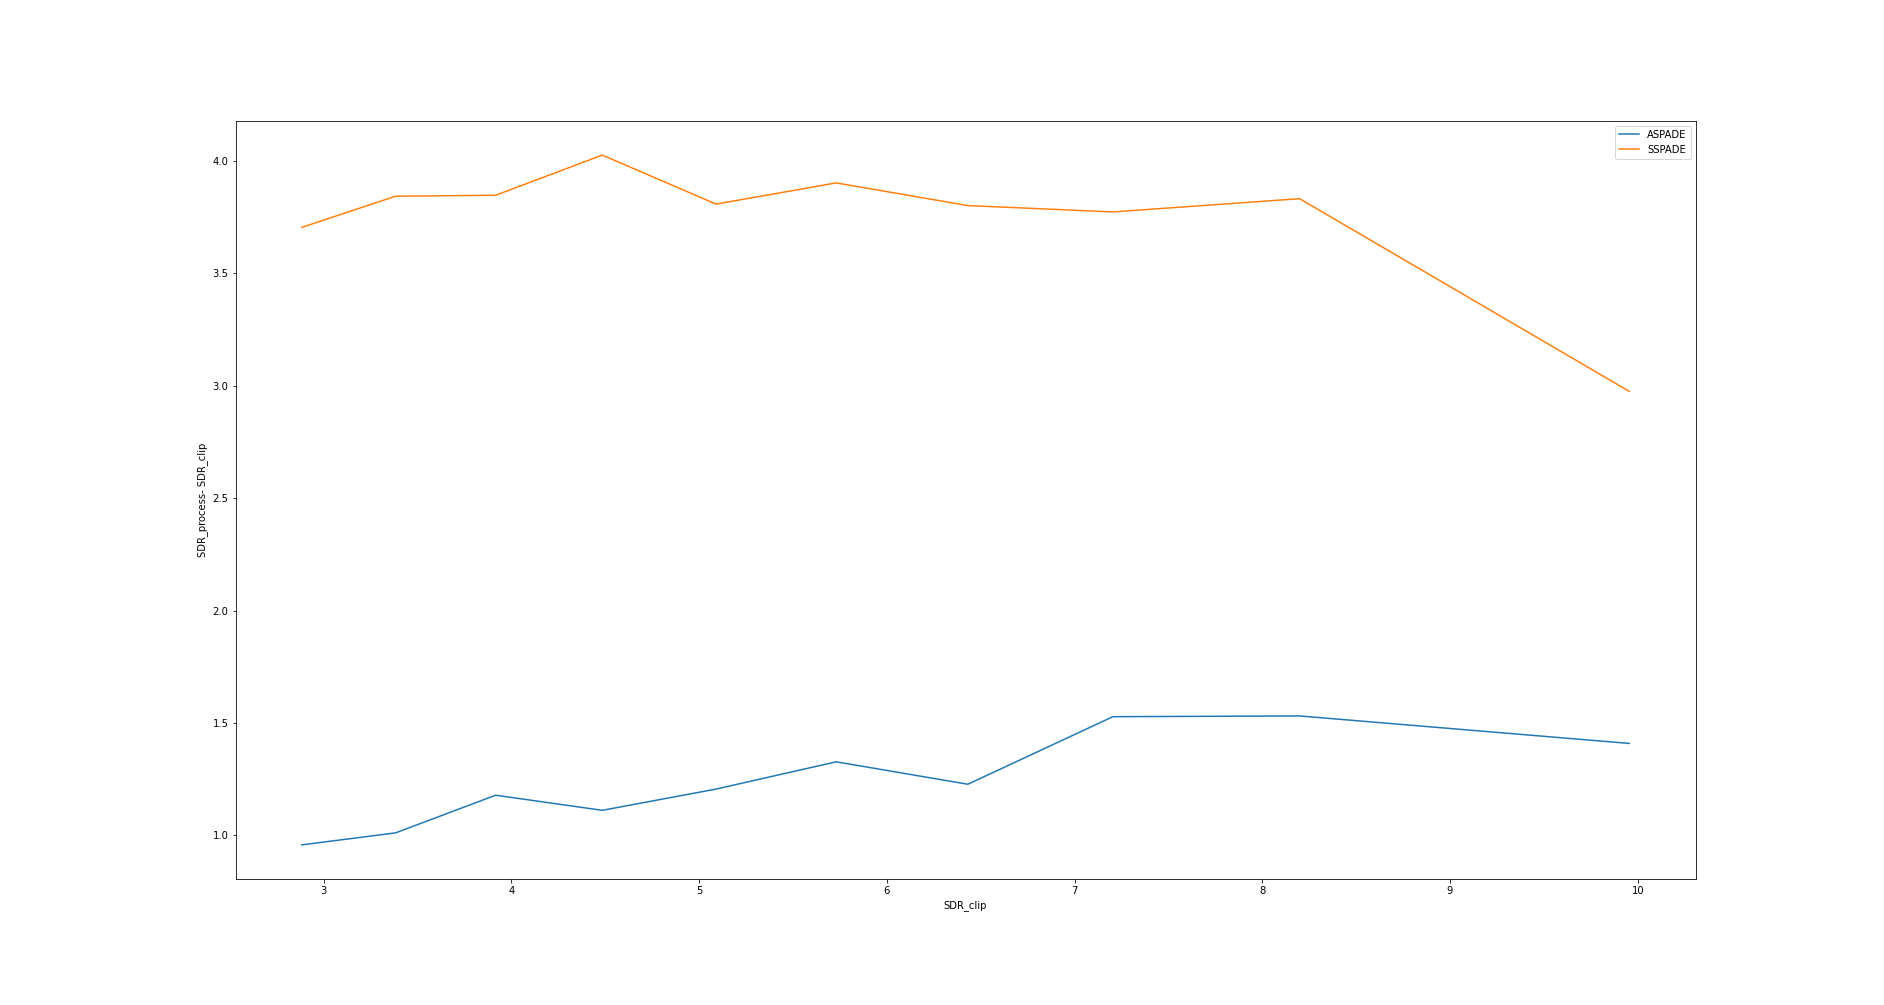
\includegraphics[width=\textwidth]{fig/Figure_3.png}
  \caption{A-SPADE and S-SPADE compared in terms of SDR, blue: A-SPADE, orange: S-SPADE}
  \label{fig:sdr}
\end{figure*}

In the following, I used the same settings as in XX (hamming windows, 1024 samples wide and 75\% overlap). Various test soundtrack are available in the repository.

On \ref{fig:plot} we can see that the Algorithm does perform a suitable reconstruction, finding new data in the clipped region, and the non clipped regions are preserved, as expected.

On \ref{fig:sdr} I used \texttt{quintet.wav} to study how the reconstruction performs for a wide range of SDR.
To control the SDR through clipping, the threshold is choosed as a percentile value of the signal. To Speed things up, the initial sparsity is set to 100 (instead of 1 in the original article).

Figure \ref{fig:sdr} does not met the results of XX, my implementation is sadly out-performed by several order of magnitude.

\section{Conclusion}

Clearly, the expectation of quality of results is not met with my implementation. I did not take enough time to produced a reliable implementation in Python. Others have done a much better job, and in the survey article XX,  the best algorithm (SPADE being among these) yields results that are almost undistinguishible from the original, unclipped audio tracks. Future research on this problem will probably be towards realtime declipping, and its applications.

Apart from the current state of the art, SPADE algorithm may also be refined, and tuned further. An potentially good track to explore lay in the frame operator and the sampling of the time-frequency grid.

\nocite{*}
\printbibliography
\end{document}
